\section{Results}


We first checked for serial dependence using ACF and PACF. For General Ukraine Aid Stance polarization, the autocorrelation at lag 2 was 0.373, with the partial autocorrelation reaching the same lag at 0.352. No other lags exceeded its band. For the PBI, the lag 3 autocorrelation came on top at 0.365, while no lags exceeded its band. Figure 1 displays both diagnostics. These diagnostic suggested serial dependence at lag 2 and potentially lag 3 for General Aid Stance polarization and PBI respectively, so we applied the Hamed-Rao's adjustment appropriately for each. Nevertheless, the correction is proven neutral, as the correction factor was 1 for both series, suggesting that none of the detrended rank reached significant autocorrelation; only the raw series did. Thus, our significance from Mann-Kendall is not more permissive than the uncorrected test. To also account for autocorrelation when fitting and searching for the better model that described the temporal trajectory of polarization and PBI, we also incorporated an estimation of autoregressive error process alongside the regime level in the shift model. After modeling the relevant autocorrelations for each series, Ljung-Box tests at lag 8 detected no remaining autocorrelation for polarization (Q = 9.31, p = 0.157) and the Party Brand Index (Q = 11.77, p = 0.162).



\begin{figure}[htbp]
\centering
\caption{Autocorrelation and Partial Autocorrelation of Polarization and PBI}
\label{fig:1}
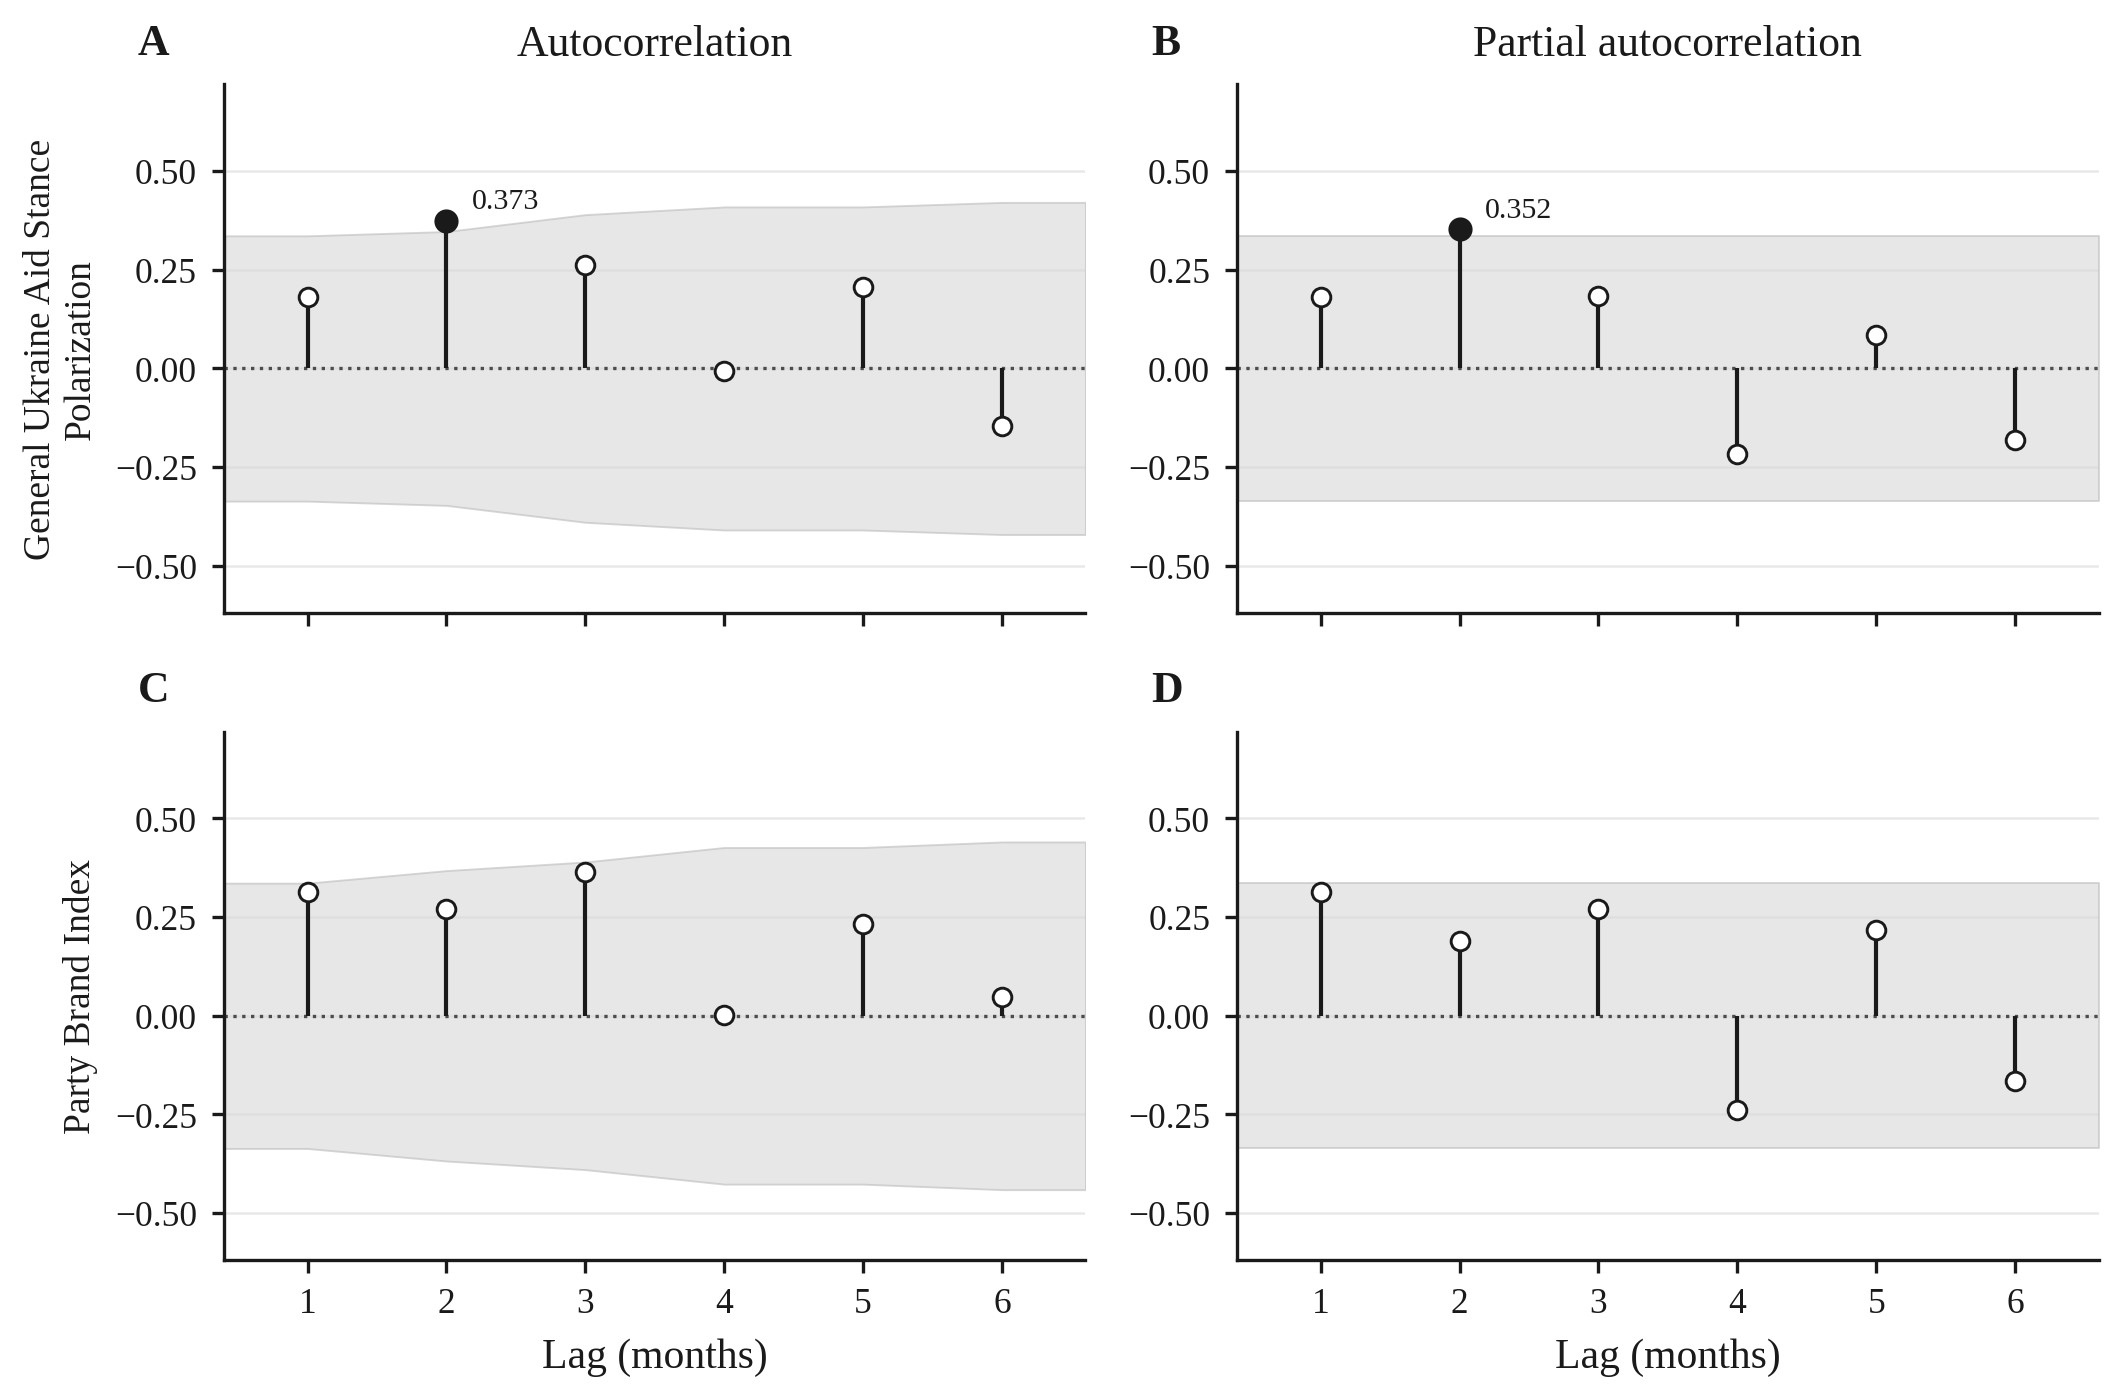
\includegraphics[width=\textwidth]{figures/figure_1_acf_pacf.png}

\begin{minipage}{\textwidth}\footnotesize \textit{Note.} Diagnostics computed on the raw monthly series before trend testing. Shaded regions are approximate 95\% reference bands: cumulative Bartlett bands for the autocorrelation function and $\pm1.96/\sqrt{N}$ for the partial function. Filled markers fall outside the band. $N = 34$ months.\end{minipage}
\end{figure}


Dimensional coverage varied as expected given differences in how frequently news discourse addresses each aspect of the Ukraine aid debate. General Ukraine Aid Stance had the highest non-NA rate at 62.6\%, comprising 23,364 scored sentences and averaging approximately 687 sentences per month. Ukraine Characterization captured 27.3\% of sentences (n = 10,198; 300 sentences/month), while Resource Allocation captured 20.2\% (n = 7,523; 221 sentences/month). Threat Priority had the lowest coverage at 9.8\% (n = 3,650; 107 sentences/month), as relatively few Ukraine-related sentences explicitly addressed threat prioritization. These differential rates may reflect the topical specificity of each dimension across the studied period. Separately, Democrats constituted the majority of politician mentions across all dimensions, ranging from 56.1\% in General Aid Stance to 74.9\% in Threat Priority, suggesting that Democrats were mentioned much more frequently on news coverages.

Table 4 reports the estimates that answer RQ1, RQ2a, and RQ4. Table 5 reports the structural model comparisons for General Aid Stance polarization and PBI.


\begin{table}[htbp]
\centering
\small
\begin{threeparttable}
\caption{Decisive Temporal Estimates}
\label{tab:4}
\begin{tabularx}{\textwidth}{@{}L{1.30}L{0.95}rrrL{0.85}@{}}
\toprule
\textbf{Construct} & \textbf{Estimand} & \textbf{Estimate} & \textbf{95\% interval} & \textbf{p} & \textbf{Analysis set} \\
\midrule
General Ukraine Aid Stance polarization & Sen slope & 0.29 & [0.061, 0.59] & .006 & 34 months \\
Selected shift-only polarization structure & December 2024 - March 2022 fitted contrast & 11.71 & [9.99, 13.42] & <~.001 & Conditional on selected structure \\
Republican General Ukraine Aid Stance & Marginal Sen slope & 0.42 & [0.23, 0.67] & <~.001 & 34 months \\
Democratic General Ukraine Aid Stance & Marginal Sen slope & 0.17 & [0.065, 0.28] & .015 & 34 months \\
Republican minus Democratic change & Direct paired Sen contrast & 0.29 & [0.061, 0.59] & .006 & 561 month pairs \\
Party Brand Index & Sen slope & 0.36 & [0.15, 0.54] & .001 & 34 months \\
\bottomrule
\end{tabularx}
\end{threeparttable}
\end{table}



\begin{table}[htbp]
\centering
\small
\begin{threeparttable}
\caption{Structural Model Selection}
\label{tab:5}
\begin{tabularx}{\textwidth}{@{}L{1.15}L{0.60}L{0.90}rrL{1.05}@{}}
\toprule
\textbf{Construct} & \textbf{Role} & \textbf{Model} & \textbf{BIC} & \textbf{$\Delta$BIC} & \textbf{Estimated onset(s)} \\
\midrule
General Ukraine Aid Stance polarization & Selected & Three-shift AR(2) & 218.41 & 0.00 & 2022-09, 2023-04, 2023-09 \\
General Ukraine Aid Stance polarization & Runner-up & Four-shift AR(2) & 219.66 & 1.25 & 2022-09, 2023-01, 2023-05, 2023-09 \\
Party Brand Index & Selected & One-shift AR(0) & 215.48 & 0.00 & 2023-09 \\
Party Brand Index & Runner-up & No-shift AR(1) & 224.83 & 9.35 & None \\
\bottomrule
\end{tabularx}
\end{threeparttable}
\end{table}


\subsection{RQ1}

General Ukraine Aid Stance polarization increased significantly over the study period. Across the 34 months, the Hamed-Rao Mann-Kendall statistic was S = 185, Kendall's $\tau$ = .330, Z = 2.73, p = .006. Based on Kendall's $\tau$, we can learn that, of the 561 pairs our data allows, 373 showed a wider polarization in the later month against 188 that showed a narrower one. The Sen slope was 0.29 polarization points per month, with a 95\% rank interval of [0.061, 0.59], which suggests a rough growth of 9.6 points from March 2022 to December 2024.

Under the selected structural model, which we detail below, the fitted December 2024 polarization gap was 11.71 points larger than the fitted March 2022 gap with the 95\% structure-conditional interval of [9.99, 13.42], p < 0.001. Take this evidence with Sen slope, the two places the period increase at roughly 10 to 12 points on the 0 to 100 stance scale, a change of about 40\% against the 28.2 point level of the first regime (March 2022 to September 2022). Figure 2 Panel A shows the exact temporal trajectory with the selected regime and shift. H1a is supported.



\begin{figure}[htbp]
\centering
\caption{Temporal Trajectory of Polarization and the Party Brand Index}
\label{fig:2}
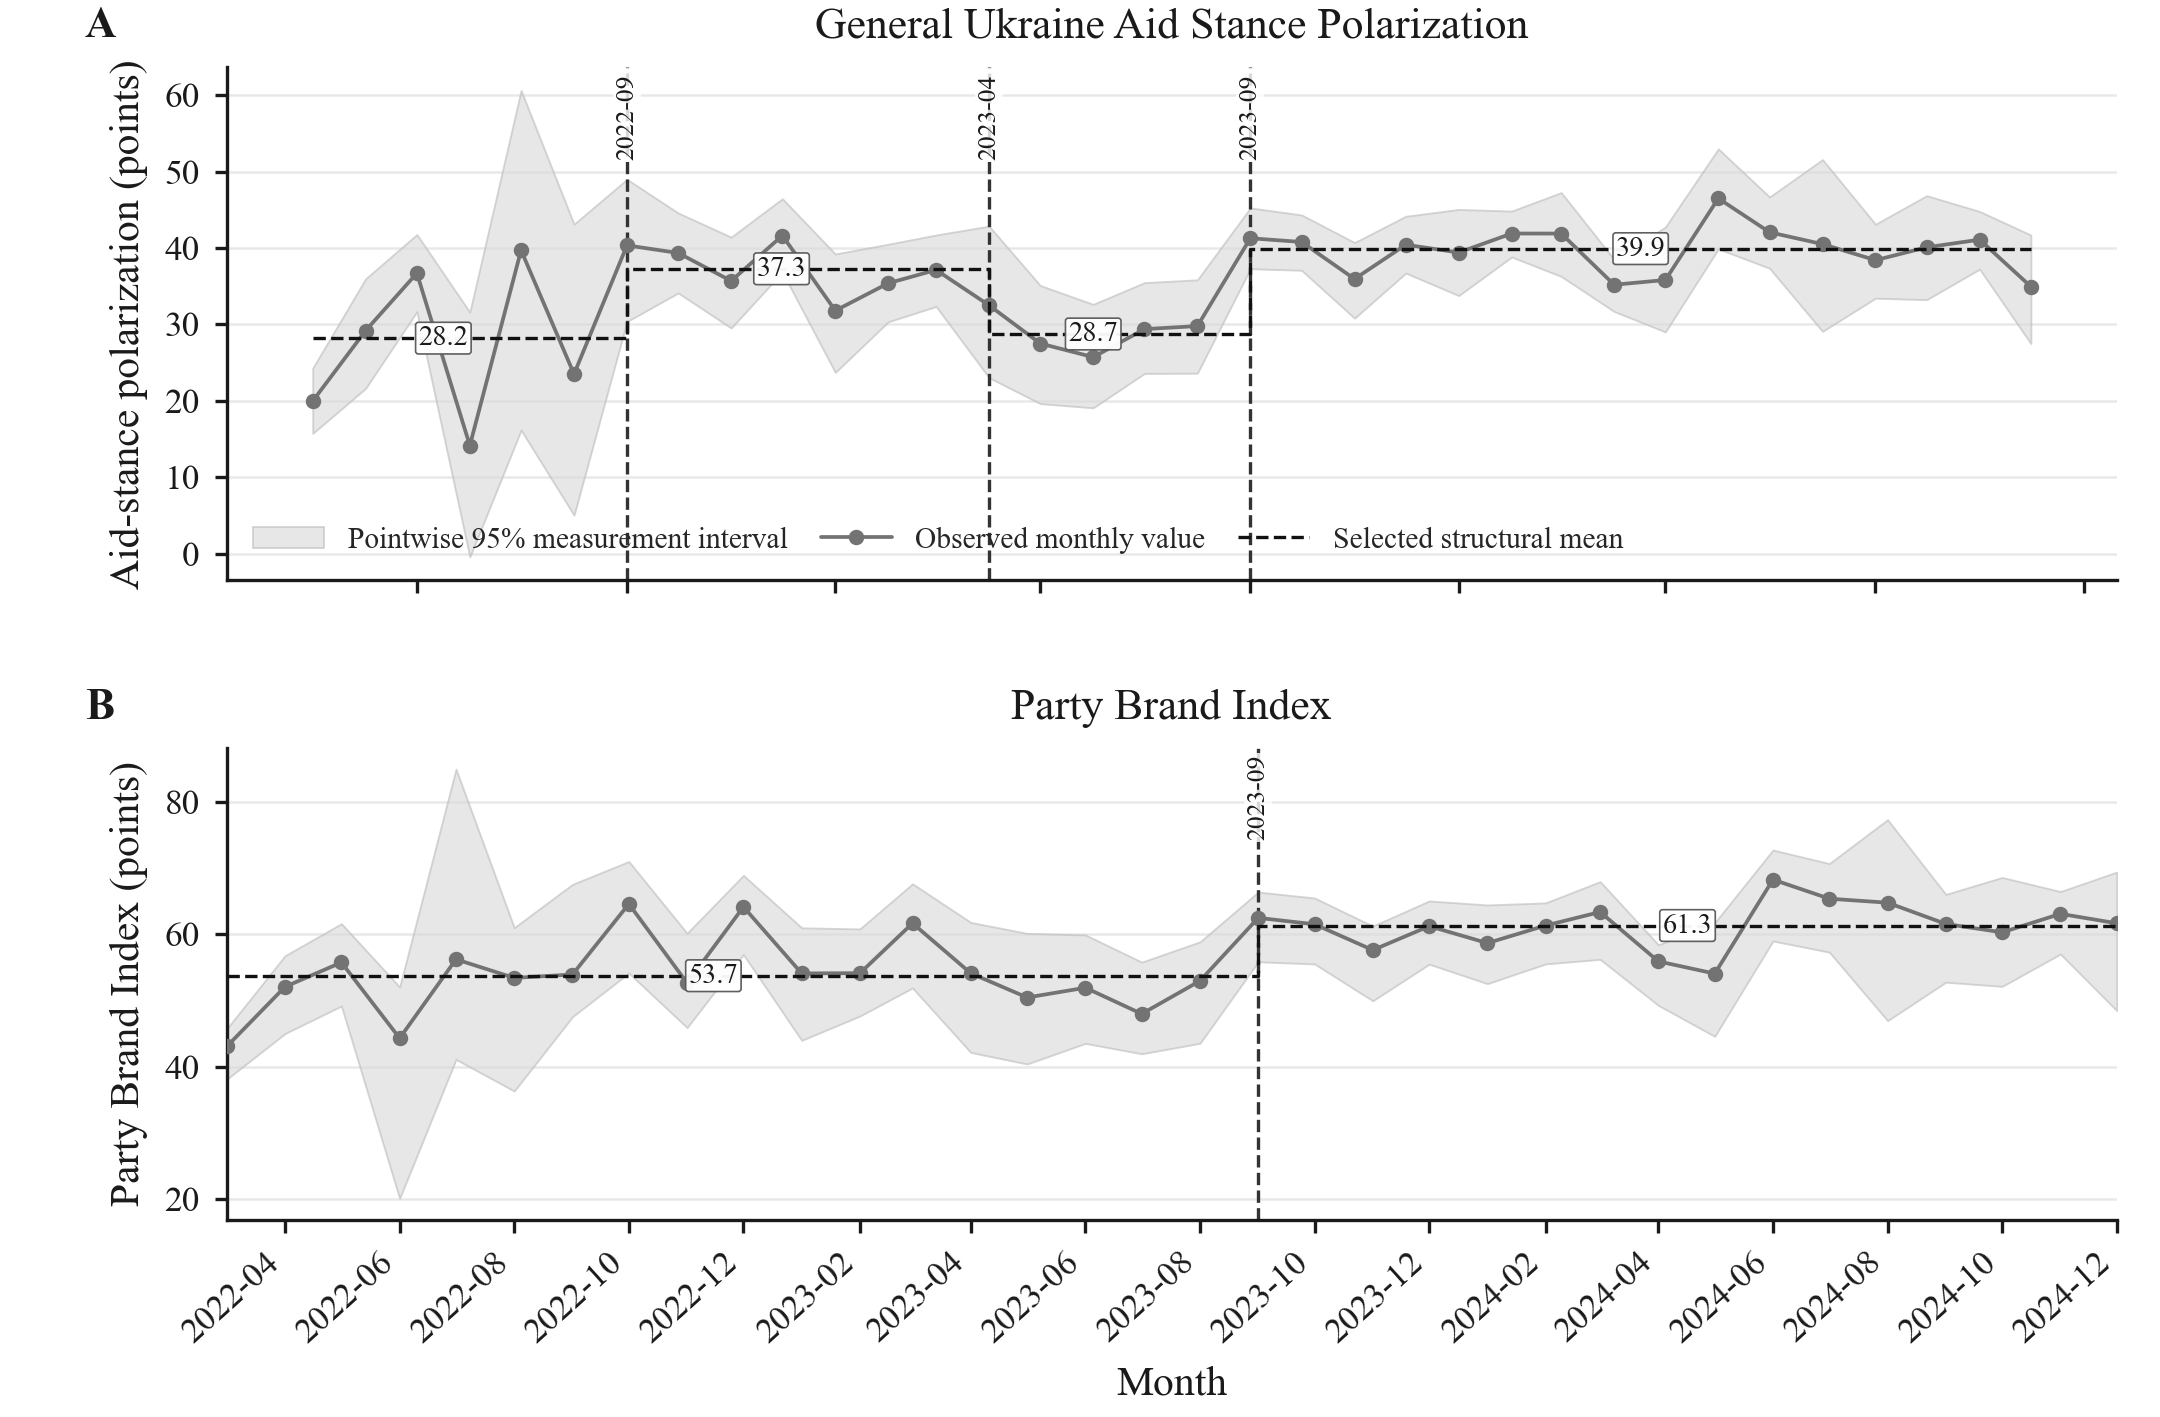
\includegraphics[width=\textwidth]{figures/figure_2_structural_development.png}

\begin{minipage}{\textwidth}\footnotesize \textit{Note.} Panel A shows General Ukraine Aid Stance polarization, discussed under RQ1. Panel B shows the Party Brand Index, discussed under RQ4. Bands are pointwise 95\% article-cluster measurement intervals, and onset lines mark estimated new-regime starts.\end{minipage}
\end{figure}


Table 6 reports the three descriptions fitted: a single gradual trend with no shifts, a set of constant levels separated by shifts at particular onset dates, and constant levels with a single gradual trend running through them. The shift-only model carried the lowest adjusted BIC at 218.41, against 228.23 by the trend-only model and 221.90 for shift-plus-trend model. The common slope in the third model was -0.019 points per month, 95\% CI[-0.21, 0.18], p = .85, so adding a trend to a model that already contains shifts contributed no additional structure.


\begin{table}[htbp]
\centering
\small
\begin{threeparttable}
\caption{Comparison of the Three Trajectory Models for Polarization}
\label{tab:6}
\begin{tabularx}{\textwidth}{@{}L{1.00}rrrrL{1.10}@{}}
\toprule
\textbf{Model class} & \textbf{Shifts} & \textbf{AR order} & \textbf{BIC} & \textbf{$\Delta$BIC} & \textbf{Estimated onset(s)} \\
\midrule
Trend only & 0 & AR(0) & 228.23 & 9.82 & None \\
Shifts only (selected) & 3 & AR(2) & 218.41 & 0.00 & 2022-09, 2023-04, 2023-09 \\
Shifts plus common trend & 3 & AR(2) & 221.90 & 3.49 & 2022-09, 2023-04, 2023-09 \\
\bottomrule
\end{tabularx}
\end{threeparttable}
\end{table}


The selected model placed onset of each regime to September 2022, April 2023, and September 2023. Its four regime level were 28.2, 37.3, 28.7, and 39.9 polarization points: the trajectory increased, fell back to its starting level, then rose again and sustained. Such pattern is what a single slope could average over and why shift model outperformed the rest. This structure also held under sensitivity tests. Minimum regime duration of 3, 4 and 5 months returned the same results. The 6-month duration retained three shifts and moved only the middle onset because April to March 2023 is a five-month regime. Nevertheless, the runner-up four-shift alternative was also competitive at $\Delta$BIC = 1.25. Nonetheless, the evidence suggests that the temporal trajectory of General Aid Stance polarization was punctuated rather than gradual. H1b is supported.

\subsection{RQ2a}

As shown in Figure 3, both party's stance has moved toward opposition, though the Republican have moved further. The Republican's marginal Sen slope was 0.42 General Aid Stance points per month (95\% CI [0.23, 0.67], p < .001), and the Democratic slope was 0.17 points per month (95\% CI[0.065, 0.28], p = .015). However, to decisively compare the movement between the two, we held both parties to the same 561 month pairs. The median of the paired Republican-and-Democratic slope difference was 0.29 per month (95\% CI[0.061, 0.59], p = 0.006). As stated in Method, this estimate is identical to the polarization Sen slope, but it does establish the fact that Republican, as reflected by news, moved further than Democrats. Therefore, H2a is supported.



\begin{figure}[htbp]
\centering
\caption{Party Stance Trajectories and Direct Paired Change}
\label{fig:3}
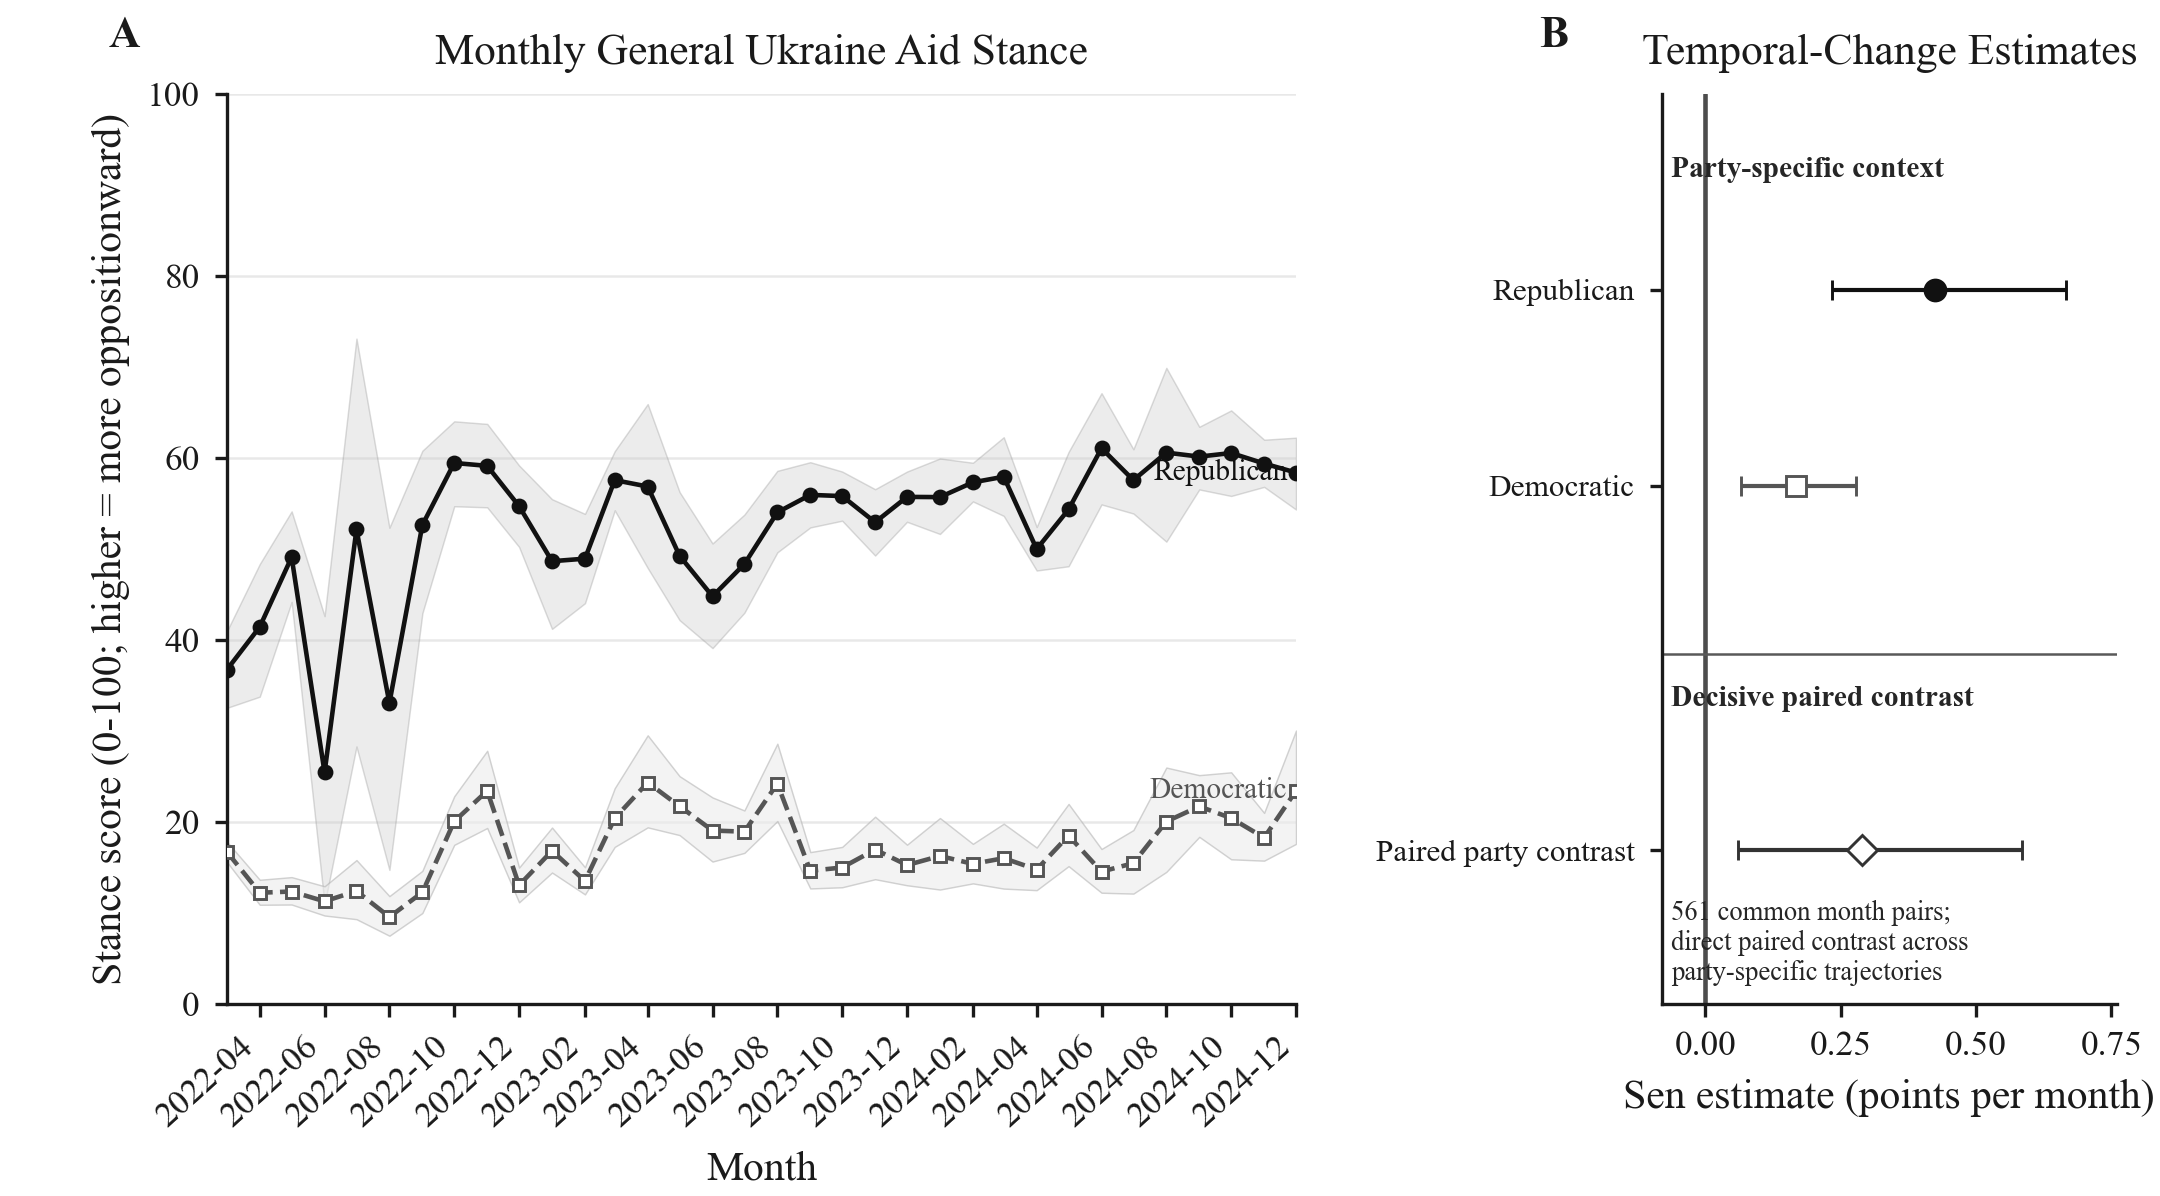
\includegraphics[width=\textwidth]{figures/figure_3_party_stance.png}

\begin{minipage}{\textwidth}\footnotesize \textit{Note.} Panel A shows monthly General Ukraine Aid Stance for each party. Panel B shows the two marginal Sen slopes and the direct paired contrast. Bands are pointwise 95\% article-cluster measurement intervals; forest intervals are 95\% Sen rank intervals.\end{minipage}
\end{figure}


\subsection{RQ2b}

The three explanatory dimensions together accounted for 29.4\% of the variation in General Ukraine Aid Stance polarization. Resource Allocation supplied the greatest contribution at 0.18, which is 61.2\% of the model R\textsuperscript{2}, followed by Ukraine Characterization at 24.3\%, and Threat Priority at 14.4\%. Table 7 reports the full decomposition. The Resource-Allocation-and-Ukraine-Characterization contrast was 0.11 (95\% CI[-0.27, 0.48]), and the Resource-Allocation-and-Threat-Priority contrast was 0.14 (95\% CI[-0.24, 0.51]). Both interval included zero. Additionally, Resource Allocation ranked first in 50.5\% of the stationary bootstrap draws, which is close to random across replicates. Therefore, while Resource Allocation did came on top as theory would suggest, H2b is not supported.


\begin{table}[htbp]
\centering
\small
\begin{threeparttable}
\caption{Descriptive General-Dominance Decomposition}
\label{tab:7}
\begin{tabularx}{\textwidth}{@{}L{0.95}L{1.25}rrL{1.05}@{}}
\toprule
\textbf{Row role} & \textbf{Construct or contrast} & \textbf{Estimate} & \textbf{Share of model R\textsuperscript{2}} & \textbf{Simultaneous 95\% interval} \\
\midrule
Observed contribution & Resource Allocation & 0.180 & 61.2\% & --- \\
Observed contribution & Ukraine Characterization & 0.072 & 24.3\% & --- \\
Observed contribution & Threat Priority & 0.042 & 14.4\% & --- \\
Dependence-preserving contrast & Resource Allocation minus Ukraine Characterization & 0.109 & --- & [-0.265, 0.482] \\
Dependence-preserving contrast & Resource Allocation minus Threat Priority & 0.138 & --- & [-0.235, 0.511] \\
\bottomrule
\end{tabularx}
\end{threeparttable}
\end{table}


\subsection{RQ3}

Neither party's General Aid Stance polarization showed significant relationship with within-party coherence. We selected the model with lowest BIC of 498.58 that contained independently monthly errors, over the alternative with AR(1) and BIC of 500.92. This choice was held fixed across measurement panels. Since a lower IQR indicates greater within-party coherence, greater coherence with higher polarization would appear as a negative coefficient. Table 8 reports the coefficient for centered polarization and centered time, split by party.


\begin{table}[htbp]
\centering
\small
\begin{threeparttable}
\caption{Model of Within-Party Coherence}
\label{tab:8}
\begin{tabularx}{\textwidth}{@{}L{0.75}L{0.95}rrL{1.00}rL{1.05}@{}}
\toprule
\textbf{Party} & \textbf{Term} & \textbf{$\beta$} & \textbf{SE} & \textbf{95\% CI} & \textbf{p} & \textbf{Measurement 95\% CI} \\
\midrule
Republican & Intercept & 39.89 & 1.73 & [36.36, 43.42] & < .001 & [36.40, 42.35] \\
Republican & Polarization & 0.049 & 0.291 & [$-$0.545, 0.643] & .868 & [$-$1.022, 0.466] \\
Republican & Time & $-$0.77 & 0.208 & [$-$1.189, $-$0.342] & < .001 & [$-$0.951, $-$0.166] \\
Democratic & Intercept & 20.15 & 0.99 & [18.12, 22.17] & < .001 & [18.43, 21.32] \\
Democratic & Polarization & $-$0.10 & 0.167 & [$-$0.444, 0.237] & .538 & [$-$0.460, 0.101] \\
Democratic & Time & 0.17 & 0.119 & [$-$0.078, 0.408] & .176 & [$-$0.032, 0.383] \\
Contrast & Republican minus Democratic polarization & 0.15 & 0.373 & [$-$0.609, 0.914] & .685 & [$-$0.889, 0.628] \\
\bottomrule
\end{tabularx}
\end{threeparttable}
\end{table}



The Democratic coefficient was negative at $\beta$ = -0.10 (95\% CI[-0.44, 0.24]) with a measurement-propagated interval of [-0.46, 0.10]. The Republican coefficient was positive at $\beta$ = 0.049 (95\% CI[-0.55, 0.64]) with a measurement-propagated interval of [-1.02, 0.47]. Both party's CI included zero, suggesting that we cannot reliably confirm if there is a significant positive relationship between polarization and within-party coherence. Additionally, the Republican coefficient also changed sign under the AR(1) model, reaching -0.26, suggesting that its direction and magnitude is not stable across error structure. Therefore, H3 is not supported.

Turning to the time coefficient, however, depicts a different pattern than the polarization coefficients. While Republican's within-party coherence increased significantly, Democrat did not, it instead decreased slightly. Republican raw IQR fell by 0.77 points per month (SE = 0.21, p < 0.001, 95\% CI[-1.19, -0.34]), the Democratic raw IQR increased by 0.17 points per month (SE = 0.12, p = 0.18, 95\% CI [$-$0.078 0.41]).

\subsection{RQ4}

The PBI ranged from 43.03 in March 2022 to 68.23 in June 2024, averaging at 57.29 across the studied period. It increased significantly, with a Sen slope of 0.36 index points per month (95\% CI[0.15, 0.54], p = .001), which accumulates to roughly a 12-points rise. The structure that best described the trajectory of PBI is simpler than polarization. The selected model places a single onset in September 2023, BIC = 215.48, as shown in the Panel B of Figure 2. Its regime levels were 53.72 before the onset and 61.30 after the onset, with an increase of 7.58 PBI points. The runner-up was a no-shift AR(1) model that is 9.35 BIC points higher.

\subsection{Summary of findings}

Overall, the polarization of General Ukraine Aid Stance increased substantially from March 2022 to December 2024, with this increase taking the form of three persistent level shifts rather than steady growth. The paired comparison showed larger Republican than Democratic movement toward opposition, suggesting that most of the growth in polarization is driven by Republican movement. Resource Allocation accounted for the most of the contemporaneous variations in the General Aid Stance polarization. Lastly, the PBI increased and moved to a higher regime level from September 2023, and there was no significant correlation between polarization and either party's within-party coherence within the studies period.

